\documentclass[12pt,reqno,letter]{article} %\bibliographystyle{jasanum}

\usepackage[utf8x]{inputenc}
\usepackage{amsmath,amsfonts,amssymb,amscd,amsthm,xspace}
\usepackage{subfigure}
\usepackage{graphicx}
\usepackage{hyperref}
\usepackage{capt-of}
\renewcommand\refname{Bibliography}
\usepackage{setspace}
\usepackage{natbib}
\bibliographystyle{apalike}
\usepackage{parskip}
% smaller margins:
\usepackage{fullpage}
\usepackage{tabu}
\usepackage{array}
\usepackage[
singlelinecheck=false % <-- important: left-aligns captions
]{caption}

%\renewcommand{\baselinestretch}{2}
% \renewcommand{\section}[1]{\medskip \addtocounter{section}{1}\raggedright 
%     \textbf{\Roman{section}. \ #1}\medskip \setcounter{subsection}{0}
%    \setlength{\parindent}{5ex}
% }
% \renewcommand{\subsection}[1]{\medskip \addtocounter{subsection}{1}\raggedright
%    \textbf{\Alph{subsection}. \ #1} \medskip \setcounter{subsubsection}{0}  
%    \setlength{\parindent}{5ex}
% }



\renewcommand{\thesection}{\Roman{section}}
\renewcommand{\thesubsection}{\thesection.\Alph{subsection}}


 \renewcommand{\bibsection}{\medskip \raggedright  \textbf{References}
    \medskip}

\renewcommand{\bibnumfmt}[1]{\textbf{{#1}.}\ \ }


 \setlength{\parindent}{5ex}
 \setlength{\paperwidth}{8.5in}
 \setlength{\textwidth}{6.5in}
 \setlength{\oddsidemargin}{0in}
 \setlength{\evensidemargin}{0in}

   


%\newcommand{\cp}{   \ensuremath{v_{\text{P}}}}
%\newcommand{\vp}{   \ensuremath{v_{\text{x}}}}
%\newcommand{\vs}{   \ensuremath{v_{\text{S}}}}
%\newcommand{\vsh}{  \ensuremath{v_{\text{y}}}}
%\newcommand{\vsv}{  \ensuremath{v_{\text{z}}}}
%\newcommand{\MPa}{  \ensuremath{\text{MPa}}}
%\newcommand{\ms}{   \ensuremath{ \frac{\text{m}}{\text{s}}}}
%\newcommand{\kms}{  \ensuremath{ \frac{\text{km}}{\text{s}}}}
%\newcommand{\mh}{   \ensuremath{ \frac{\text{m}}{\text{h}}}}
%\newcommand{\kHz}{  \ensuremath{\text{kHz}}}
 
\begin{document}
% 

%\title[Structural monitoring with traffic recordings ]{Structural monitoring of a highway bridge using passive noise recordings from street traffic }
\title{An Event Database for Rotational Seismology}

\author{Johannes Salvermoser, Bryant Chow, C\'{e}line Hadziioannou, Sarah Hable, Lion Krischer, Catalina-M. Ramos-Domke, Joachim Wassermann, Ulrich Schreiber, Andre Gebauer, and Heiner Igel}

%\email[]{hadzii@geophysik.uni-muenchen.de}
%\homepage[]{Your web page}
%\thanks{}
%\altaffiliation{}
%\affiliation{Department for Earth- and Environmental Sciences\\ Ludwig-Maximilians-University\\ Theresienstrasse 41, 80333 Munich
 %Author's affiliation
%}
% 
% 
% 
%\date{\today}
% 

\begin{center}

\textbf{An Event Database for Rotational Seismology}

\vspace{6em}
Johannes Salvermoser\footnote{email: jsalvermoser@geophysik.uni-muenchen.de}, Bryant Chow, C\'{e}line Hadziioannou, Sarah Hable, Lion Krischer, Catalina Marlene Ramos Domke, Joachim Wassermann, Ulrich Schreiber, Andre Gebauer, and Heiner Igel
\vspace{3em}

Department for Earth- and Environmental Sciences\\ Ludwig-Maximilians-University\\ Theresienstrasse 41, 80333 Munich


%Pacs: 43.40.Le, 43.40.Ph, 43.20.Jr, 43.20.Fn

\end{center}

\begin{abstract}
We introduce the new event database for rotational seismology. On this website the user can access 17000+ processed global earthquake events starting in 2007. For each event, we provide waveform and processing plots for the seismometer station at Wettzell and its G-ring ring laser, as well as extracted values in a separate file. Tutorials and illustrated processing guides are available and are ready to be used for processing on the user-side. The aim is to promote the use of rotational ground motion data by offering data for many events and giving access to well-explained ObsPy-based sample code. 
\end{abstract}
%\newpage
% 
%\pacs{%
%43.40.Le, 43.40.Ph, 43.20.Jr, 43.20.Fn
%}
% 
%\keywords{Non-Destructive Testing \sep Concrete Bridge \sep Passive Image Interferometry \sep Cross-correlation \sep Structural Health Monitoring \sep Coda Wave Interferometry}
%\maketitle must follow title, authors, abstract, \pacs, and \keywords
%\maketitle
% 
%%%%%%%%%%%%%%%%%%%%%%%%%%%%%%%%%%%%%%%%%%%%%%%%%%%%%%%%%%%%%%%%%%%%%%%%%%%%%%
%%%%%%%%% SECTION INTRODUCTION
%%%%%%%%%%%%%%%%%%%%%%%%%%%%%%%%%%%%%%%%%%%%%%%%%%%%%%%%%%%%%%%%%%%%%%%%%%%%%%
% 
\section{Introduction}
Since the beginning of the 20th century, seismology has been dominated by one type of observation: translational ground motions (usually measured as three orthogonal components: N-S, E-W, vertical). In the past two decades, due to the emerging ring laser gyroscope development and its calibration to high sensitivities \citep{Stedman1995,Stedman1997,Schreiber2003, Schreiber2004} for geodetic applications, rotational ground motions have become available as a new observable in seismology.
\cite{AkiRichards2002} pointed out that -~to reconstruct complete ground motions~- rotational motions should also be observed.
\\ 
In this regard, \cite{McLeod1998, Pancha2000} have shown that vertical rotation rate and transverse acceleration are in phase and \cite{Igel2005,Igel2007} and \cite{Kurrle2010} found that from amplitude ratios of these measurements in a single point, it is possible to estimate dispersion curves of Love waves generated by (teleseismic) earthquakes.\\
Until then, another aspect, the determination of the event source direction, was only feasible with seismic array measurements (e.g. beam-forming). However, \cite{Igel2007} deduced a straight-forward approach to infer the source direction (=backazimuth) from  collocated broadband seismometer and ring laser recordings using a cross-correlation grid search.\\
The idea of consistently processing ring laser (rotational motion) recordings and giving the opportunity to use the resulting information lead to the initiation of the presented event database, with two main intentions.

\noindent
The first main goal is to make processed rotation data publicly available in order to promote its usage and significance for seismological applications. In this context, we built up an event database containing event plots and separate metadata files including valuable extracted event parameters.\\
The second goal is to show how rotational waveforms (e.g. vertical component rotation rates from Wettzell \textbf{G-Ring}) can be accessed and processed. For this purpose, we provide tutorials in terms of open source Jupyter Notebooks \citep{Perez2007} which graphically and interactively present the basic processing - as used for the database entries - while providing helpful background information. The notebooks are based on the seismological toolbox \textbf{ObsPy} \citep{Megies2011,Krischer2015}.

\noindent
\begin{figure}[htp!]
	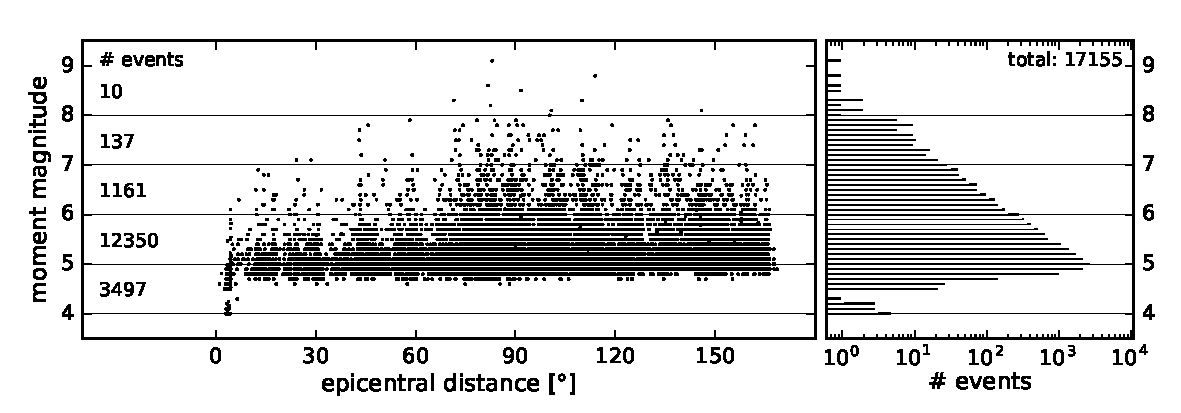
\includegraphics[width=\textwidth]{dist_mag_merged.pdf}
	\caption{Distribution of the processed events from July 2007 to July 2016 by distance and magnitude [left] and number of events per magnitude in 0.1-steps [right].}
	\label{fig:mag_dist}
\end{figure}
Currently, we process data provided by a single station, the Wettzell Geodetic Observatory in S-E Germany. The 4 x 4 m G-Ring ring laser, located there, measures the Sagnac-interference at very high resolution: until 2009 at $\approx60\frac{prad}{s}\sqrt{Hz^{-1}}$ and since 2009 at $12\frac{prad}{s}\sqrt{Hz^{-1}}$ \citep{Schreiber2013}. This yields a sensitivity to rotations around the vertical axis, that is high enough to record even teleseismic events at reasonable signal-to-noise ratio.
Translational ground motions are measured parallel to that using a collocated (dist. $\approx250m$) STRECKEISEN STS-2 broadband seismometer which is the station WET of the German regional network. So far, since 2007 more than 17000 events have been processed (see figure~\ref{fig:mag_dist}) using this station's data. As soon as continuous rotational motion recordings of other ring lasers are available, we will include them in our database to also allow inter-station comparison.\\
% 
%%%%%%%%%%%%%%%%%%%%%%%%%%%%%%%%%%%%%%%%%%%%%%%%%%%%%%%%%%%%%%%%%%
% 
\section{Website}
\label{sec:website}

The website provides the visitor with a graphical user interface of the database as well as additional information and links to topic-related projects (see figure~\ref{fig:website}).
Upon defining filter parameters (time period, magnitude, latitude/longitude), the user obtains a map representation of the specified available event catalog. In the zoomable world map, the earthquake events markers are sized and colored according to the earthquake’s moment magnitude and source depth, respectively. This is intended to help find the desired event more quickly.
By clicking on the event markers, the user opens a popup menu yielding a short description of the event by means of source time, magnitude and depth. The menu also contains links to a couple of images for the automatically processed waveform data of rotational and translational ground motions. These images display:

\begin{itemize}
	\item[1.] Event information
	\item[2.] Waveform comparison (4 different time windows)
	\item[3.] Parameter estimation (Love wave phase velocity, backazimuth)
	\item[4.] P-coda analysis
\end{itemize}
\begin{figure*}[!htp]
\centering
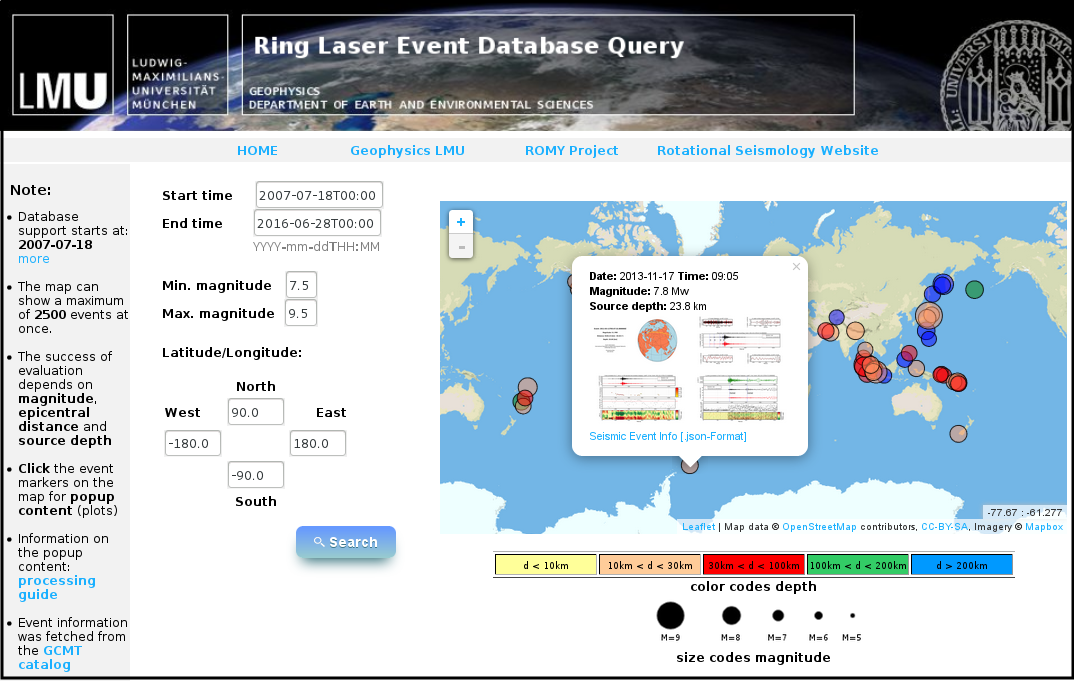
\includegraphics[width=\textwidth]{webpage_framed.png}
\caption{Web view of the event database for rotational seismology.}
\label{fig:website}
\end{figure*}
\noindent
Finally, the menue links to a metadata parameter file in the easily (machine-) readable json-dictionary format. This dictionary contains all event and data fetching information and most importantly processed parameters such as  peak values (displacement, acceleration, rotation rate, correlation), signal-to-noise ratios, mean phase velocities (+ STDs), estimated and theoretical backazimuth.
The aim of creating this file is to publicly provide event characteristics that were processed consistently and can be used for further (statistical) analysis.\\
In order to make the processing transparent and the produced plots understandable, we include a downloadable 5-page processing guide  and Python-ObsPy based example code snippets. Additionally, \textbf{Jupyter notebooks}, linked to this website, interactively explain the processing steps from data download and instrument correction to phase velocity and backazimuth estimation.
%
%%%%%%%%%%%%%%%%%%%%%%%%%%%%%%%%%%%%%%%%%%%%%%%%%%%%%%%%%%%%%%%%%%%%%%%%%%%%%%
%%%%%%%%% SECTION PROCESSING
%%%%%%%%%%%%%%%%%%%%%%%%%%%%%%%%%%%%%%%%%%%%%%%%%%%%%%%%%%%%%%%%%%%%%%%%%%%%%%
%
\section{Processing}
\label{sec:processing}
\subsection{Pre-processing}
The event database is automatically updated on a daily basis. That means hard-coded Python-scripts keep the database up-to-date running on a fixed schedule. The scripts are fed by event quick solutions provided by the Global Centroid Moment Tensor (GCMT) catalog \citep{Dziewonski1981, Ekstroem2012}. This catalog contains global earthquake events featuring moment magnitudes $M_w > 4.5$. The event-/data-download and processing is based on different ObsPy routines.\\
After fetching the QuakeML-format event information (origin time, epicenter, depth, etc.), raw ring laser and collocated seismometer waveforms are downloaded via a FDSN (“International Federation of Digital Seismograph Networks”) web service.
The pre-processing of the downloaded seismic data streams is determined by the source-receiver distance (cf. table~\ref{table:params}).
\begin{table}[htp]
\caption{Pre-processing parameters}
	\vspace{0.3cm}
	\begin{tabular}{l|ccccc}
	& \begin{tabular}{@{}c@{}}\textbf{distance}\\ \textbf{range}\end{tabular}& \begin{tabular}{@{}c@{}}\textbf{lowpass}\\ \textbf{cutoff}\end{tabular} & \begin{tabular}{@{}c@{}}\textbf{resampling}\\\textbf{decimation factor}\end{tabular} & \begin{tabular}{@{}c@{}}\textbf{cross-correlation}\\\textbf{window length}\end{tabular}& \begin{tabular}{@{}c@{}}\textbf{microseism}\\ \textbf{bandstop}\end{tabular}\\
	\hline
	\textbf{close} & 0\textdegree$\le d \le$3\textdegree & 4 Hz & 2 & 3 s & - \\
	\hline
	\textbf{local} & 3\textdegree$\le d \le$10\textdegree & 2 Hz & 2 & 5 s & - \\
	\hline
	\textbf{tele} & $d >$10\textdegree & 1 Hz & 4 & 120 s & 5 s - 12 s \\  
	
	\end{tabular}
	\label{table:params}
\end{table} 
It starts with the removal of the seismometer’s impulse response, the derivation of ground acceleration \textbf{nm/s²} from the measured ground velocity and the scaling of the ring laser's rotation rate measurements to \textbf{nrad/s}. The traces are low-pass filtered to decrease the impact of high frequency body waves and the ambient cultural noise. Furthermore, for teleseismic events, a bandstop-filter (5-12s) is applied to reduce the effect of the secondary microseism ($\approx$~7s period) which is more prominent than the primary microseism \citep{Hadziioannou2012} and can cause shifts in our backazimuth estimation especially for Mid- to South-Atlantic events for the case of the Wettzell station location.\\
Further procedure details are important to understand the automatic generation of the four popup-images (see section~\ref{sec:website} above) and the subsequent processing steps: 
to determine the theoretical arrival times for the P- and S-wave windows we use the ObsPy-\textbf{TauP} routine using IASP91 travel time tables. The surface wave arrivals are  based on interpolated IASP91 surface wave travel times. The processing leading to the subplots of image 3 is described in the subsections \ref{subsec:pv} and \ref{subsec:be}.
It is notable, that for the P-coda analysis (image 4), shorter time windows (local: 2s; teleseismic: 5s) are used for the cross-correlation analysis to show that there is a (weak) signal of P- or SV-converted S$_H$ waves in the high-frequency P-coda and thus before the theoretical S-wave arrival.

%
\subsection{Love wave phase velocity estimation}
\label{subsec:pv}
\begin{figure*}[!htp]
\centering
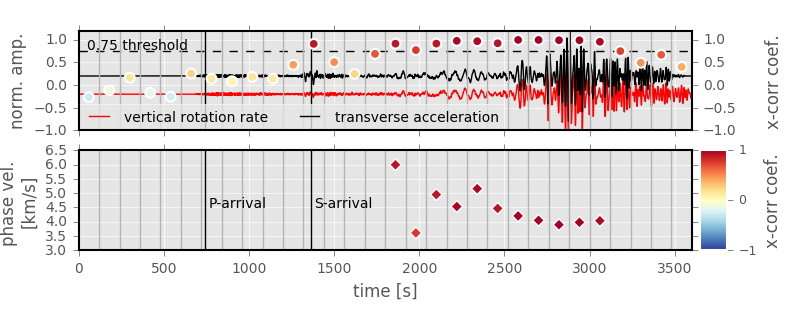
\includegraphics[width=\textwidth]{paper_plot1.png}
\caption{Visualization of the sliding window phase velocity estimation for the M9.0 $T\overline{o}hoku$ earthquake 03/11/2011. For each of the time windows, a cross-correlation is performed between vertical rotation rate and transverse acceleration [top]. We estimate phase velocities for windows associated with correlation coefficients (\textbf{CC}) larger than 0.75 and later than S-waves [bottom].}
\label{fig:phase_vel}
\end{figure*}
\noindent
In order to derive Love wave phase velocities, the observed and pre-processed signals are compared analogous to \cite{Igel2005}. Under the assumption of a transversely polarized plane wave, the vertical rotation rate $\dot{\Omega}_z$ and transverse acceleration $a_t$ are in phase and the amplitudes are related by: 
\begin{equation}
	\frac{a_t}{\dot{\Omega}_z} = -2c
\end{equation}
where c is the (apparent) horizontal phase velocity. In a first step, we therefore rotate (by the theoretical BAz) the horizontal acceleration components (North-East) in the source-receiver plane to radial-transverse to obtain a phase-match with the vertical rotation rate. The transverse acceleration and vertical rotation rate traces are then divided into sliding windows of equal size depending on the epicentral distance of the event (see table~\ref{table:params}).
For each of these windows, a zero-lag normalized cross-correlation analysis is applied to $a_t$ and $\dot{\Omega_z}$ to check the coherence between the two waveforms (figure~\ref{fig:phase_vel} [top]). The resulting cross-correlation coefficient (CC) is used as a quality criterion for the determination of the phase velocities. For windows with CC $>$ 0.75, the horizontal phase velocity c is calculated by inserting peak values of $a_t$ and $\dot{\Omega_z}$ in the relation of equation~1 (figure~\ref{fig:phase_vel} [bottom]).
For broadband traces and high waveform coherence (=high quality signal) we will obtain an impression of the dispersive behaviour of Love waves immediately by looking at the temporal evolution of the phase velocity. That means the dominant frequency of Love waves increases with time while phase velocities decrease.

\subsection{Backazimuth Estimation}
\label{subsec:be}
Similar to the phase velocity estimation and analogous to \cite{Igel2007}, we investigate sliding windows throughout the signal to catch the evolution of the signal source direction.  Again, the traces are split into windows according to table~\ref{table:params}.
For each window, we estimate the direction of the signal in the two pre-processed traces (vert. rot. rate \& transv. acc.) employing a grid search optimization algorithm. 
%
\begin{figure*}[!htp]
\centering
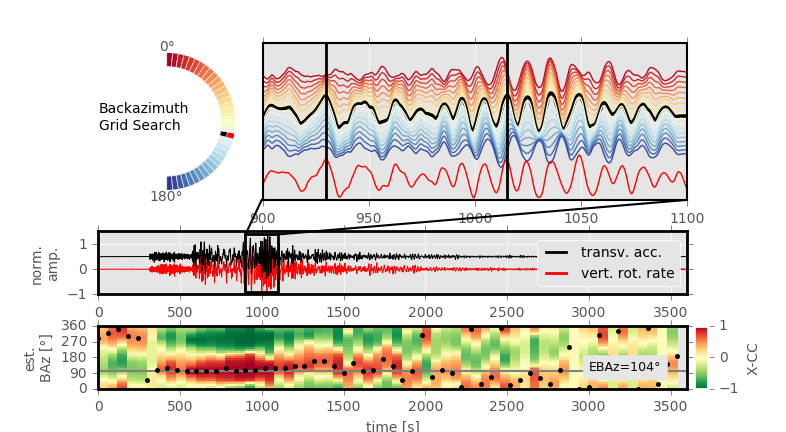
\includegraphics[width=\textwidth]{pp_Baz_paperready.png}
\caption{Illustration of the backazimuth estimation workflow at the example of the M7.1 Turkey quake 10/23/2011. (a) The grid search algorithm loops through all possible source directions (red to blue) in 1\textdegree -steps, cross-correlating the two traces of $a_t$ and $\dot{\Omega}_z$, shown in (b). In (c) for each time window, the BAz-value related to maximum correlation is displayed as a black dot. Here, red color displays correlation, while green is anti-correlation of the traces for the specific BAz angle. Estimated (EBAz) and theoretical backazimuth (TBAz) are indicated by the gray solid line.}
\label{fig:baz}
\end{figure*}
%
The routine loops through all possible backazimuth directions (0° to 360°) in 1°- steps, for each step rotates the horizontal component acceleration (N-E) by the specified BAz-angle and then cross-correlates it with the vertical rotation rate. The process is illustrated in figure \ref{fig:baz} [a] where a color range is assigned to different BAz rotation angles.  The CCs are maximal for a rotation from N-E to radial-transverse which is equivalent to rotating in the direction of the strongest signal source (note: transv. acc. (black) and vert. rot. rate (red) are in phase).\\ 
In practice, only windows reaching 90\% correlation after rotation are considered in the estimation of the final BAz value, which is the average of the associated (CC$>$0.9) BAz results (solid line in figure \ref{fig:baz} [c]). 
Discrepancies between the theoretical and estimated BAz in combination with higher CCs on the estimated BAz side may indicate deviations of the Love wave path in the source-receiver plane. Thus, it might suggest heterogeneities/scatterers of similar size as the dominant wavelength along the direct great-circle wave path.\\

\section{Conclusions}
We want to promote the processing and use of rotational motion recordings by providing processed waveform plots and parameters as well as illustrated real data processing examples using ObsPy. Event parameters and waveform plots of more than 17000 earthquakes since 2007 can be downloaded and used for statistical analysis. For example, this allows investigating the peak rotational ground motions as a function of magnitude and distance and the analysis of azimuthal effects on the wave field.\\
In the future, we plan on including recordings of additional ring lasers such as the ones located at the observatories of Pi$\tilde{n}$on Flat (USA, GEOsensor, \cite{Schreiber2003b}), Gran Sasso (IT, GINGERino, \cite{Ortolan2016}, Christchurch (NZ, \cite{Schreiber2003}) and the 4-component ring laser in Fuerstenfeldbruck (DE, ROMY = Rotational Motions in Seismology) to be installed in 2016. We also plan to include measurements of array derived rotations and portable rotation sensors as soon as they are available.
%%%%%%%%%%%%%%%%%%%%%%%%

%\section*{Tables}


\section*{Acknowledgments}
We would like to thank ... Wettzell Geodetic Observatory (TUM) ... European Research Council (ROMY) ??file reference ... Emmy-Noether Program of the
DFG (HA7019/1-1)



\label{Bibliography}
%\begin{thebibliography}{99}
\bibliography{Bibliography_ROMY.bib}
%
%\newcommand{\enquote}[1]{``#1''}
%\providecommand{\bibinfo}[2]{#2}
%\providecommand{\noopsort}[1]{}
%\providecommand{\switchargs}[2]{#2#1}
%


%\end{thebibliography}


\newpage

\section*{Data and Resources}
The Global Centroid Moment Tensor Project database was searched using www.globalcmt.org (last accessed 5 August 2015)\\

\noindent
The Global Centroid Moment Tensor Project database was searched using www.globalcmt.org (last accessed 5 August 2015)\\


\noindent
\section*{figure captions}

\noindent
Figure 1: -

\noindent
Figure 2: -

\noindent
Figure 3: -


\noindent   
\noindent   

\end{document}
%
% ****** End of file jasatmpl.tex ******
